% \pretextual

% ---
% Capa
% ---
%-------------------------------------------------------------------------
% Comentário adicional do PPgSI - Informações sobre a ``capa'':
%
% Esta é a ``capa'' principal/oficial do trabalho, a ser impressa apenas 
% para os casos de encadernação simples (ou seja, em ``espiral'' com 
% plástico na frente).
% 
% Não imprimir esta ``capa'' quando houver ``capa dura'' ou ``capa brochura'' 
% em que estas mesmas informações já estão presentes nela.
%
%-------------------------------------------------------------------------
\imprimircapa
% ---

% ---
% Folha de rosto
% (o * indica que haverá a ficha bibliográfica)
% ---

% \imprimirfolhaderosto*

% ---

% ---
% Inserir a autorização para reprodução e ficha bibliografica
% ---

%-------------------------------------------------------------------------
% Comentário adicional do PPgSI - Informações sobre o texto da 
% ``autorização para reprodução e ficha bibliografica'':
%
% Página a ser usada apenas para Dissertação/Tese (tanto na versão original 
% quanto na versão corrigida).
%
% Solicitar a ficha catalográfica na Biblioteca da EACH. 
% Duas versões devem ser solicitadas, em dois momentos distintos: uma vez 
% para a versão original, e depois outra atualizada para a versão 
% corrigida.
%
% Atenção: esta página de ``autorização para reprodução e ficha 
% catalográfica'' deve ser impressa obrigatoriamente no verso da folha de 
% rosto.
%
% Não usar esta página para Qualificação.
%
% Substitua o arquivo ``fig_ficha_catalografica.pdf'' abaixo referenciado 
% pelo PDF elaborado pela Biblioteca
%
%-------------------------------------------------------------------------

% \begin{fichacatalografica}
%     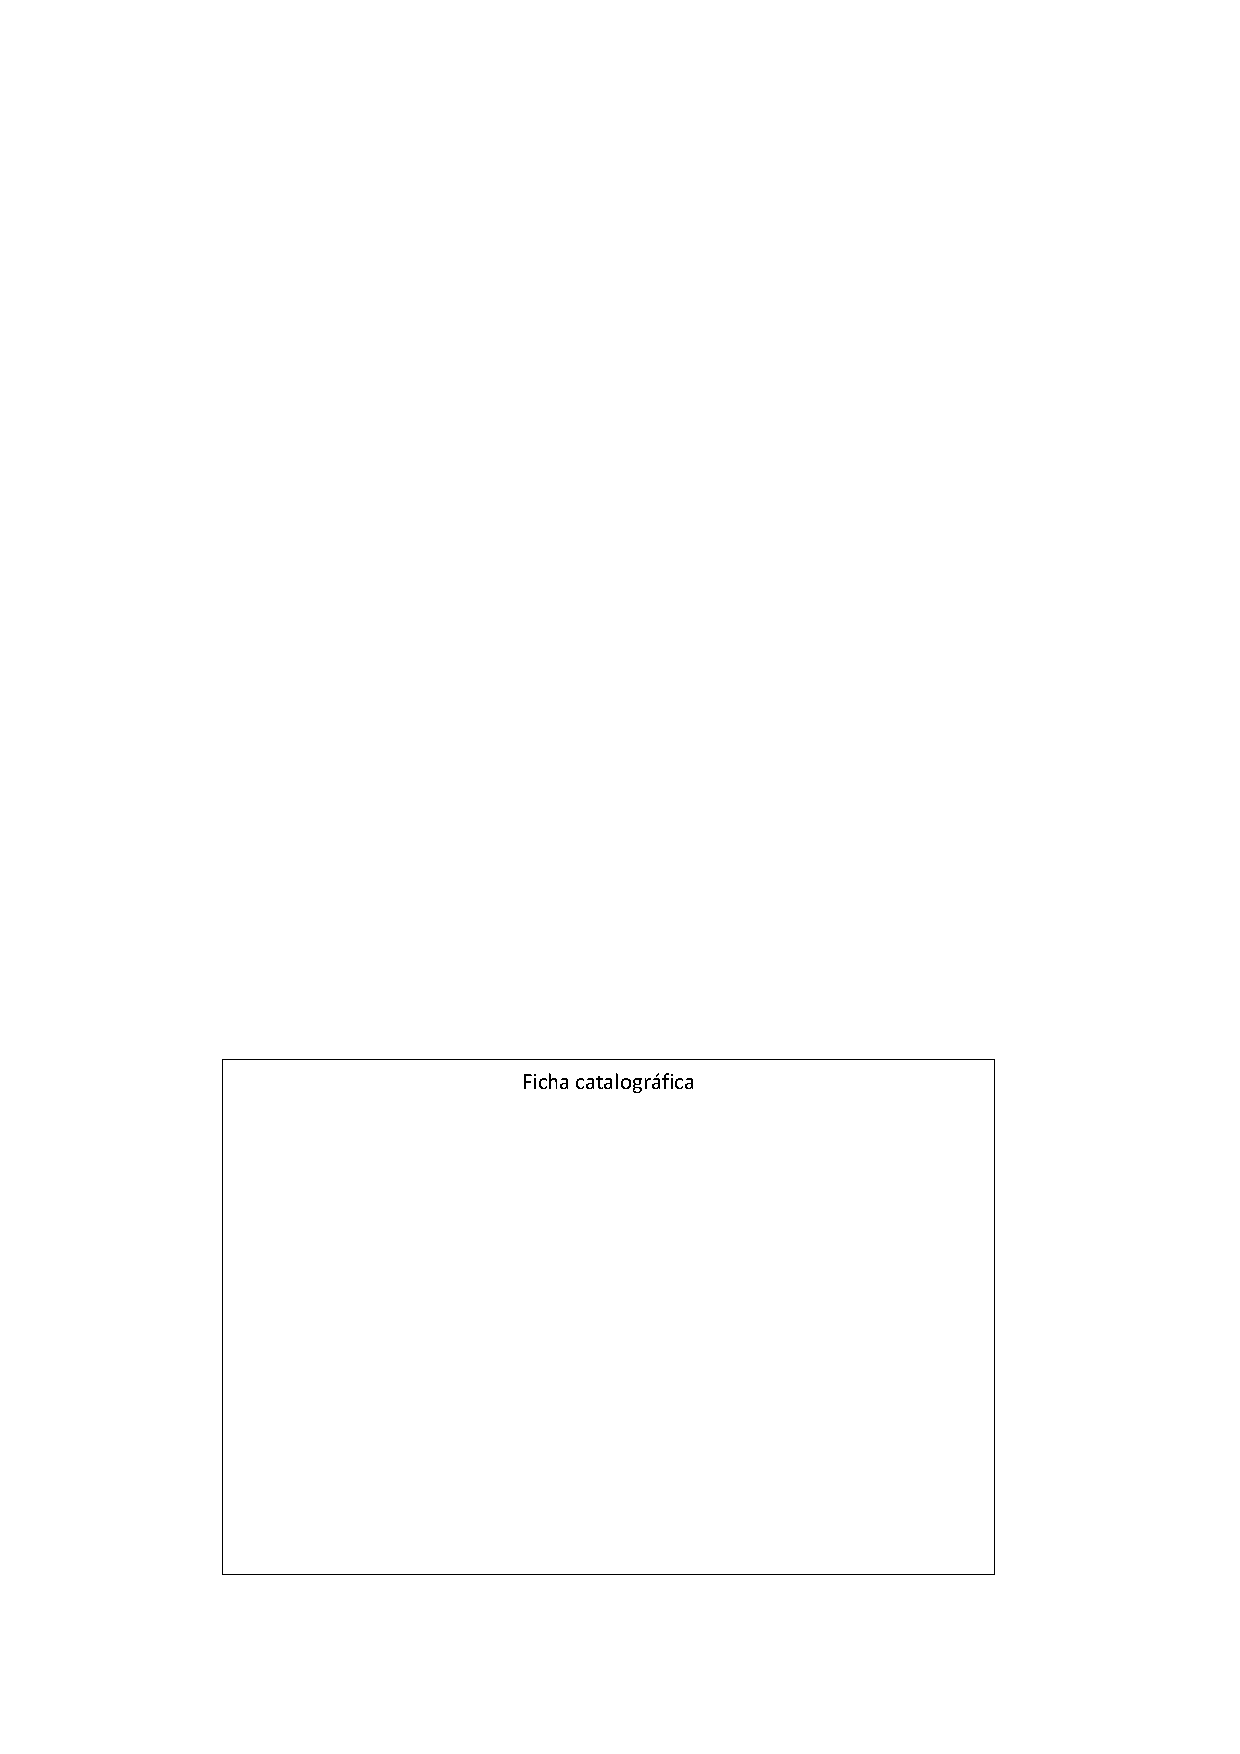
\includepdf{exemplos/fig_ficha_catalografica.pdf}
% \end{fichacatalografica}

% ---
% Inserir errata
% ---
%-------------------------------------------------------------------------
% Comentário adicional do PPgSI - Informações sobre ``Errata'':
%
% Usar esta página de errata apenas em casos de excepcionais, e apenas 
% para a versão corrigida da Dissertação/Tese. Por exemplo, quando depois de
% já depositada e publicada a versão corrigida, ainda assim verifica-se
% a necessidade de alguma correção adicional.
%
% Se precisar usar esta página, busque a forma correta (o modelo correto) 
% para fazê-lo, de acordo com a norma ABNT.
%
% Não usar esta página para versão original de Dissertação/Tese.
% Não usar esta página para Qualificação.
%
%-------------------------------------------------------------------------
% \begin{errata}
% Elemento opcional para versão corrigida, depois de depositada.
% \end{errata}
% ---

% ---
% Inserir folha de aprovação
% ---

% \begin{folhadeaprovacao}

%-------------------------------------------------------------------------
% Comentário adicional do PPgSI - Informações sobre ``Folha da aprovação'':
%
% Página a ser usada apenas para Dissertação/Tese.
%
% Não usar esta página para Qualificação.
%
% Substituir ``Fulano de Tal'' pelo nome completo do autor do trabalho, com 
% apenas as iniciais em maiúsculo.
%
% Substituir ``___ de ______________ de ______'' por: 
%     - Para versão original de Dissertação/Tese: deixar em branco, pois a data 
%       pode mudar, mesmo que ela já esteja prevista.
%     - Para versão corrigida de Dissertação/Tese: usar a data em que a defesa 
%       efetivamente ocorreu.
%
% Para Tese de Doutorado: trocar "Dissertação" por "Tese".
%-------------------------------------------------------------------------
% \noindent Dissertação de autoria de Fulano de Tal, sob o título \textbf{``\imprimirtitulo''}, apresentada à Escola de Artes, Ciências e Humanidades da Universidade de São Paulo, para obtenção do título de Mestre em Ciências pelo Programa de Pós-graduação em Sistemas de Informação, na área de concentração Metodologia e Técnicas da Computação, aprovada em \rule{0.85cm}{0.5pt} de \rule{3.5cm}{0.5pt} de \rule{1.25cm}{0.5pt} pela comissão julgadora constituída pelos doutores:

% \vspace*{3cm}

% \begin{center}
%-------------------------------------------------------------------------
% Comentário adicional do PPgSI - Informações sobre ``assinaturas'':
%
% Para versão original de Dissertação/Tese: deixar em 
% branco (ou seja, assim como está abaixo), pois os membros da banca podem
% mudar, mesmo que eles já estejam previstos.
% 
% Para versão corrigida de Dissertação/Tese: usar os dados dos examinadores que 
% efetivamente participaram da defesa. 
% 
% Para versão corrigida de Dissertação/Tese: em caso de ``professora'', trocar 
% por ``Profa. Dra.'' 
% 
% Para versão corrigida de Dissertação/Tese: ao colocar os nomes dos 
% examinadores, usar seus nomes completos, exatamente conforme constam em 
% seus Currículos Lattes
% 
% Para a versão corrigida de Dissertação/Tese: remova o texto “Instituição: ”, 
% ou seja, coloque apenas/diretamente o nome da instituição, por exemplo 
% "Universidade de São Paulo" ou "Universidade Estadual de Campinas".
%
% Não abreviar os nomes das instituições.
%
% Verifique quantos membros há em sua banca, de acordo com o seu regulamento, 
% especificamente para o caso de Dissertação de Mestrado ou Tese de Doutorado, 
% e use o número correto de espaços para assinaturas.
%
%-------------------------------------------------------------------------

% \assinatura{Prof. Dr. \\ Instituição \\ Presidente}

% \assinatura{Prof. Dr. \\ Instituição}

% \assinatura{Prof. Dr. \\ Instituição}

% \assinatura{Prof. Dr. \\ Instituição}    % Incluir para bancas de tese de doutorado

% \assinatura{Prof. Dr. \\ Instituição}    % Incluir para bancas de tese de doutorado

% \end{center}
  
% \end{folhadeaprovacao}


% ---

% ---
% Dedicatória
% ---
%-------------------------------------------------------------------------
% Comentário adicional do PPgSI - Informações sobre ``Dedicatória'': 
%
% Opcional para Dissertação/Tese.
% Não sugerido para Qualificação.
% 
%-------------------------------------------------------------------------
% \begin{dedicatoria}
%    \vspace*{\fill}
%    \centering
%    \noindent
%    \textit{Escreva aqui sua dedicatória, se desejar, ou remova esta página...} 
% 	 \vspace*{\fill}
% \end{dedicatoria}
% ---

% ---
% Agradecimentos
% ---
%-------------------------------------------------------------------------
% Comentário adicional do PPgSI - Informações sobre ``Agradecimentos'': 
%
% Opcional para Dissertação/Tese.
% Não sugerido para Qualificação.
% 
% 
% Financiamentos recebidos durante o projeto de mestrado/doutorado, vindos de qualquer 
% agência de fomento, devem ser mencionados na seção de agradecimentos da dissertação/tese. 
% Isso se aplica não apenas a bolsas de estudo, mas a qualquer tipo de financiamento, 
% tais como para apoio a participação em eventos, compra de materiais, traduções etc. 
% Especificamente para financiamento da Capes, siga as instruções contidas na portaria 
% 206, de 4/set/2018; para outras agências de fomento, procure as regras apropriadas.
%
% Portaria Capes 206, de 4/set/2018: 
% http://ppgsi.each.usp.br/arquivos/Portaria_0783227_Portaria_CAPES_DOU___206_de_2018.pdf 
%
%
%-------------------------------------------------------------------------
% \begin{agradecimentos}
% Texto de exemplo, texto de exemplo, texto de exemplo, texto de exemplo, texto de exemplo, texto de exemplo, texto de exemplo, texto de exemplo, texto de exemplo, texto de exemplo, texto de exemplo, texto de exemplo, texto de exemplo, texto de exemplo, texto de exemplo, texto de exemplo, texto de exemplo, texto de exemplo, texto de exemplo, texto de exemplo, texto de exemplo, texto de exemplo.

% Texto de exemplo, texto de exemplo, texto de exemplo, texto de exemplo, texto de exemplo, texto de exemplo, texto de exemplo, texto de exemplo, texto de exemplo, texto de exemplo, texto de exemplo, texto de exemplo, texto de exemplo, texto de exemplo, texto de exemplo, texto de exemplo, texto de exemplo, texto de exemplo, texto de exemplo, texto de exemplo, texto de exemplo, texto de exemplo.

% Texto de exemplo, texto de exemplo, texto de exemplo, texto de exemplo, texto de exemplo, texto de exemplo, texto de exemplo, texto de exemplo, texto de exemplo, texto de exemplo, texto de exemplo, texto de exemplo, texto de exemplo, texto de exemplo, texto de exemplo, texto de exemplo, texto de exemplo, texto de exemplo, texto de exemplo, texto de exemplo, texto de exemplo, texto de exemplo.

% Texto de exemplo, texto de exemplo, texto de exemplo, texto de exemplo, texto de exemplo, texto de exemplo, texto de exemplo, texto de exemplo, texto de exemplo, texto de exemplo, texto de exemplo, texto de exemplo, texto de exemplo, texto de exemplo, texto de exemplo, texto de exemplo, texto de exemplo, texto de exemplo, texto de exemplo, texto de exemplo, texto de exemplo, texto de exemplo.

% Texto de exemplo, texto de exemplo, texto de exemplo, texto de exemplo, texto de exemplo, texto de exemplo, texto de exemplo, texto de exemplo, texto de exemplo, texto de exemplo, texto de exemplo, texto de exemplo, texto de exemplo, texto de exemplo, texto de exemplo, texto de exemplo, texto de exemplo, texto de exemplo, texto de exemplo, texto de exemplo, texto de exemplo, texto de exemplo.
% \end{agradecimentos}
% ---

% ---
% Epígrafe
% ---
%-------------------------------------------------------------------------
% Comentário adicional do PPgSI - Informações sobre ``Epígrafe'': 
%
% Opcional para Dissertação/Tese.
% Não sugerido para Qualificação.
% 
%-------------------------------------------------------------------------
% \begin{epigrafe}
%     \vspace*{\fill}
% 	\begin{flushright}
% 		\textit{``Escreva aqui uma epígrafe, se desejar, ou remova esta página...''\\
% 		(Autor da epígrafe)}
% 	\end{flushright}
% \end{epigrafe}
% ---

% ---
% RESUMOS
% ---

% resumo em português
\setlength{\absparsep}{18pt} % ajusta o espaçamento dos parágrafos do resumo
\begin{resumo}

%-------------------------------------------------------------------------
% Comentário adicional do PPgSI - Informações sobre ``referência'':
% 
% Troque os seguintes campos pelos dados de sua Dissertação/Tese (mantendo a 
% formatação e pontuação):
%   - SOBRENOME
%   - Nome1
%   - Nome2
%   - Nome3
%   - Título do trabalho: subtítulo do trabalho
%   - AnoDeDefesa
%
% Mantenha todas as demais informações exatamente como estão.
% 
% [Não usar essas informações de ``referência'' para Qualificação]
%
% Para Tese de Doutorado: trocar "Dissertação (Mestrado em Ciências)" por "Tese (Doutorado em Ciências)".
%-------------------------------------------------------------------------
\begin{flushleft}
SANTOS, Alexandre Farias.
\textbf{Efeitos de dados artificiais em classificadores de deep learning}: uma abordagem baseada em mapas de atenção \imprimirdata. \pageref{LastPage} f. Dissertação (Mestrado em Ciências) – Escola de Artes, Ciências e Humanidades, Universidade de São Paulo, São Paulo, 2024.
\end{flushleft}

O desenvolvimento de modelos de aprendizado de máquina é sem dúvidas um dos grandes marcos tecnológicos do nosso presente momento na história, a disponibilização de diferentes tipos de conjuntos de dados se tornou fundamental para a construção de novas ferramentas e tecnologias que impactam cada vez mais nossas vidas. Todavia a escassez de dados, ou a natureza improvável de alguns fenômenos são fatores limitantes na construção de modelos mais sofisticados e complexos como as redes neurais profundas. Para resolver este problema, diferentes tipos de modelos generativos foram desenvolvidos nos últimos anos, conseguindo resultados promissores na sintetização de dados artificiais. No entanto, a avaliação da utilidade e confiabilidade de dados artificiais não é uma tarefa trivial e exige um alto rigor científico dado seu potencial de utilização. Neste trabalho, propõe-se a utilização de métodos de explicabilidade por meio de mapas de atenção aplicados em redes neurais artificiais para trazer luz as capacidades dos modelos treinados em dados artificiais e avançar no estabelecimento de boas práticas para a avaliação destes modelos.

Palavras-chaves: Redes geradoras adversárias. Modelos de difusão. Classificação Binária. Aprendizado Profundo. Mapas de atenção.
\end{resumo}

% resumo em inglês
%-------------------------------------------------------------------------
% Comentário adicional do PPgSI - Informações sobre ``resumo em inglês''
% 
% Caso a Qualificação ou a Dissertação/Tese inteira seja elaborada no idioma inglês, 
% então o ``Abstract'' vem antes do ``Resumo''.
% 
%-------------------------------------------------------------------------
\begin{resumo}[Abstract]
\begin{otherlanguage*}{english}

%-------------------------------------------------------------------------
% Comentário adicional do PPgSI - Informações sobre ``referência em inglês''
% 
% Troque os seguintes campos pelos dados de sua Dissertação/Tese (mantendo a 
% formatação e pontuação):
%     - SURNAME
%     - FirstName1
%     - MiddleName1
%     - MiddleName2
%     - Work title: work subtitle
%     - DefenseYear (Ano de Defesa)
%
% Mantenha todas as demais informações exatamente como estão.
%
% [Não usar essas informações de ``referência'' para Qualificação]
%
%-------------------------------------------------------------------------
\begin{flushleft}
SANTOS, Alexandre Farias. \textbf{Effects of artificial data on deep learning classifiers}: a
attention map-based approach. \imprimirdata. \pageref{LastPage} p. Dissertation (Master of Science) – School of Arts, Sciences and Humanities, University of São Paulo, São Paulo, 2024. 
\end{flushleft}

The development of machine learning models is without a doubt one of the greatest technological milestones of our present moment in history, the availability of different types of data sets has become fundamental for the construction of new tools and technologies that increasingly impact our lives. However, the scarcity of data, or the unlikely nature of some phenomena, are limiting factors in the construction of more sophisticated and complex models such as deep neural networks. To solve this problem, different types of generative models have been developed in recent years, achieving promising results in synthesizing artificial data. However, evaluating the usefulness and reliability of artificial data is not a trivial task and requires high scientific rigor given its potential. In this work, we propose the use of explainability methods through attention maps applied to artificial neural networks to shed light on the capabilities of models trained on artificial data and advance the establishment of good practices for evaluating these models.

Keywords: Generative Adversarial Networks. Diffusion models. Binary Classification. Deep Learning. Attention Maps.
\end{otherlanguage*}
\end{resumo}

% ---
% ---
% inserir lista de figuras
% ---
\pdfbookmark[0]{\listfigurename}{lof}
\listoffigures*
\cleardoublepage
% ---

% ---
% inserir lista de algoritmos
% ---
% \pdfbookmark[0]{\listalgorithmname}{loa}
% \listofalgorithms
% \cleardoublepage

% ---
% inserir lista de quadros
% ---
\pdfbookmark[0]{\listofquadrosname}{loq}
\listofquadros*
\cleardoublepage


% ---
% inserir lista de tabelas
% ---
\pdfbookmark[0]{\listtablename}{lot}
\listoftables*
\cleardoublepage
% ---

% ---
% inserir lista de abreviaturas e siglas
% ---
%-------------------------------------------------------------------------
% Comentário adicional do PPgSI - Informações sobre ``Lista de abreviaturas 
% e siglas'': 
%
% Opcional.
% Uma vez que se deseja usar, é necessário manter padrão e consistência no
% trabalho inteiro.
% Se usar: inserir em ordem alfabética.
%
%-------------------------------------------------------------------------
\begin{siglas}
  \item[RNA] Redes neurais artificiais
  \item[MLP] Multilayer perceptron
  \item[DL] Deep learning
  \item[GAN] Generative adversarial networks
  \item[DM] Difussion models
\end{siglas}
% ---

% ---
% inserir lista de símbolos
% ---
%-------------------------------------------------------------------------
% Comentário adicional do PPgSI - Informações sobre ``Lista de símbolos'': 
%
% Opcional.
% Uma vez que se deseja usar, é necessário manter padrão e consistência no
% trabalho inteiro.
% Se usar: inserir na ordem em que aparece no texto.
% 
%-------------------------------------------------------------------------
% \begin{simbolos}
%   \item[$ \Gamma $] Letra grega Gama
%   \item[$ \Lambda $] Lambda
%   \item[$ \zeta $] Letra grega minúscula zeta
%   \item[$ \in $] Pertence
% \end{simbolos}
% ---

% ---
% inserir o sumario
% ---
\pdfbookmark[0]{\contentsname}{toc}
\tableofcontents*
\cleardoublepage
% ---
